\documentclass{article}
\usepackage{hyperref}
\usepackage{amsmath,amssymb}
\usepackage{graphicx}
\usepackage{caption}
\usepackage{subcaption}
\usepackage{color}
\usepackage[section]{placeins}
\renewcommand{\thesubsection}{\thesection.\alph{subsection}}
\usepackage{listings}

\title{Validation and Uncertainty Quantification Proposal for a
Solar-driven Vortex Apparatus} 
\author{Nicholas Malaya\\ Department of Mechanical Engineering \\
University of Texas at Austin}  
\date{}

\begin{document}
\maketitle
\newpage

\section{Introduction}


Renewable energy is critical to our environmental, economic, and
national security. Demand for energy is on the rise, as is our national
reliance on fossil fuel-based power plants for the bulk of our
electricity generation. There is a critical need for safe, clean, and
cost-effective alternatives to coal, such as wind, solar, hydroelectric,
and geothermal power\cite{arpa-e}. These technologies would reduce carbon dioxide
emissions and help position the U.S. as a leader in the global renewable
energy industry. This proposal details a validation plan to build
confidence in a numerical investigation for the design and optimization
of a novel device for renewable, clean energy generation. 

Much of the solar energy incident on the Earth's surface is absorbed
into the ground, which in turn heats the air layer above the surface.
This buoyant air layer contains considerable gravitational potential
energy. The basic idea behind this engineering approach is to convert the 
potential energy in this buoyant air layer to kinetic energy in an
anchored vortex, and to use that kinetic energy to drive a
vertical-axis turbine coupled with an electric generator in order to
produce electrical power. The mechanism is much like that of a naturally
occurring ``dust devil'' with baroclinic generation of vorticity in a
vertically stratified, ground-heated air layer producing a columnar vortex. 

With nearly one-third of global land mass covered by deserts, there are huge
untapped regions for capturing solar heat (about 200 W/$m^2$ averaged over
a 24-hour day, and up to 1000 W/$m^2$ peak).  The available power is
competitive in magnitude with worldwide power generation from fossil
sources. If successful, this could result in a low-cost, scalable
approach to electrical power generation that could create a new class of
renewable energy ideally suited for arid low-wind regions. 

The SoV phenomena has already been demonstrated in an experimental setup
by our partners at Georgia Tech. The simulation effort intends to utilize
Computational Fluid Dynamics (CFD) to simulate this Solar-Driven Vortex
(SoV). These computer simulations are intended to discover the optimal
system configuration for a range of scenarios and system sizes. The
results of these simulations will be used as input for the design of a
pilot site in Mesa, Arizona, and eventually, over a range of
scenarios and system sizes. 

In order for these simulations to be generally useful, they must first
be validated against existing experimental data and high fidelity
simulations. These models will then explore regimes and scales where no
experimental measurements presently exist. Characterizing the
uncertainty of predictions resulting from extrapolation is a critical
component in enabling reliable assessments of field performance of the
SoV, as it will guide the commercialization strategy of the product. 

This report provides a ``validation roadmap'' detailing the process by
which an analysis of the uncertainties inherent to this
problem may be characterized.  It will begin with a discussion of the
physics scenario and the mathematical model, as well as detailing the
reliability of each submodel and the systems inputs. We will then
discuss the validation of these models against existing experimental
data and high fidelity simulations. Finally, we will formulate a Bayesian
analysis for a sub-problem, to serve as a representative example of a
probabilistic analysis applied to this project.  

%
%
%
\section{Problem Definition}

\begin{figure}[h]
 \begin{center}
  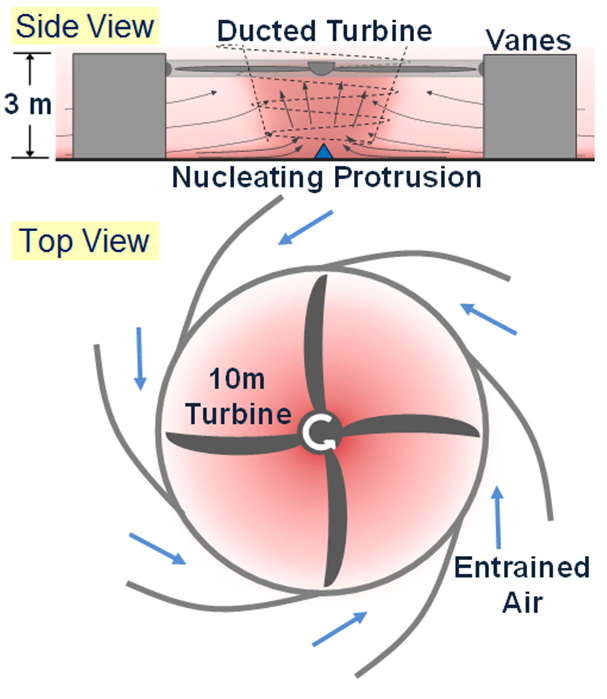
\includegraphics[width=.5\linewidth]{figs/power_generation.png}
   \caption{The Sov facility, showing the vanes, rotor and anchoring
   protrusion, as well as the buoyancy-driven vortex used to drive the
   turbine.}
   \label{facility}
  \end{center}
\end{figure}

The simulations are designed to both mimic the notional SoV experimental
facility as well as identify optimal configurations for future
designs. The general system configuration is depicted in Figure
\ref{facility}. 

Notice several important components of this device. First, ``vanes''
along the sides of the apparatus, designed to entrain outside air and
impart angular momentum. It is not known what configuration and design
of these vanes will lead to optimal dust-devil generation. Thus, these
vanes may have various configurations, varying in the number used, the
length, height, angle of attack. The vanes may also be straight, or
curved.  Next, the ducted turbine above the flow is also a critical design
component. This turbine is designed to extract energy from the flow,
without distrupting/destroying the vortex. Finally, it is desirable to
economically optimize the entire configuration scale by considering both
the power generation, cost of materials, difficulty and expense of
maintainance, etc. 

In addition to the system configuration, it is important to consider the
effect of local conditions on SoV performance. Characterizing the impact
of variations in ambient conditions on the SoV will guide the
commercialization strategy of the product, by determining optimal
install locations across the country. It is therefore desirable to have models
that are capable of accounting for variation in field conditions, such as solar
input, cross-winds and topography. Furthermore, it is expected that 
large ``farms'' of SoVs (akin to the wind and solar farms for wind
turbines 
and photovoltaics, respectively) may be used by commercial or
utility-scale energy generation. In order for this to be effective, 
the inter-unit spacing must also be optimized, as a single SoV collects
from a large area. These computations will guide commercialization
planning, where decision-makers will need to assess optimum unit size,
spacing, and geographic location for utility-scale deployment.  

%
% 2) A complete mathematical specification of the mathematical model
%   (i.e. the equations), with documentation of the basis for the
%   model, what aspects are reliable theory that need not be questioned
%   in the context of this problem, and what aspects are not as
%   reliable (i.e. embedded models), and what is known about how these
%   aspects of the model could be wrong or inaccurate.
%
%
\section{Mathematical Specification}



%
% 
%3) Identification of all parameters in the model, the available
%   information about these parameters and what is known about their
%   uncertainty.
%
%
\section{Model Parameter Specification}

The most significant parameterization in the model comes through the
stabilization parameter. Stabilization is necessary for Finite Element
Methods for fluid flows\cite{franca1992stabilized}. The choice and
design of the stability parameter is a crucial ingredient to ensure the
solution converges. However, the stability parameter also introduces
numerical dissipation, which in addition to altering the solution in a
manner inconsistent with the physical simulation regime, can also
cover-up other discrepancies that might exist in the code. 

Our choice of parameter is guided by a similar numerical
study\cite{Becker2002428} of a compressible flow at low mach number with
convection driven by a large temperature. 

However, significant uncertainties still exist. The discretization in
the study only was made with bilinear and biquadratic finite elements. 
While it also used Newton iterations to solve the nonlinear problem, no
time stepping was needed (as the problem was stationary). It is
additionally unclear how the different kinds of discretization and
solvers used in our present simulation may impact the scheme.

%
% 4) Identification of other inputs required for the model (e.g. initial
%   conditions, boundary conditions), and what is known about these
%   inputs for this problem, and associated uncertainties.
%
%
\section{Model Inputs}

The model inputs consistitute a very large component (arguably, the
largest source) of the uncertainty in this problem, for both the
laboratory and outdoor test cases. 

  \begin{figure}[!htb]
    \begin{center}
     \includegraphics[width = 12 cm]{figs/lab_setup.jpg}
     \caption{The laboratory set-up.}
     \label{lab}
    \end{center}
  \end{figure}

The experimental laboratory has numerous objects
in the immediate vicinity (see figure \ref{lab}) that may
obstruct/manipulate the flow. These objects may be moved or removed
during PIV data gathering. 

The laboratory simulation uses adiabatic side walls as a boundary
condition. It is unclear how much of an impact this may have on the
simulation. It is also unclear if this is a realistic boundary
condition. 

While no sensitivity analysis has been performed, it is likely that the
largest uncertainty in the laboratory simulation is a result of the
ventilation. This statement can be made because it was observed that the
heated plate on the bottom of the laboratory generated enough heat that
the room temperature began to rise significantly (30+ degrees
Celsius). This also greatly impacted the SoV performance, as the ground
to air thermal gradient drives the vortex. The laboratory uses cooling
in order to maintain temperature. They utilize two inlet HVAC ducts into
the room. While efforts have been made to characterize the level of
ventillation being used, these numbers come with non-trivial
uncertainties attached. As an example, a personal communication with one
of our experimental colleagues, 

``One vent runs continuously at 15 C with a flow rate of about 1
$m^3$/s (4-6 m/s with an approximate area of 0.2 $m^2$).''
Already, the inflow rate has a 50\% uncertainty in velocity
attached. Furthermore, while the area of the vents are given, the the
precise height and width are not. Thus, while our simulation uses square
vents, this may be inaccurate. 
It was also stated that, ``The other vent kicks on only if the
room gets about 28 degrees C.'' This statement has uncertainty attached to the
temperature at which the venting begins. Finally, ``The exit air is just
what ever leaves through/around the doors as we've blocked off all of
the out ducts.'' This also presents a challenge, as it is unclear (for
validation purposes) where one should expect the outflow to
go. \footnote{\normalsize Author note: This story related here not as a comment on
our collaborators. Rather, this is presented as an example of the challenges
and uncertainties that presently exist in this numerical investigation.}

The initial conditions in both the laboratory and the outdoor
tests are highly uncertain. The dimensions of the laboratory are
measured with a high degree of confidence, the initial temperature
in the room is not closely measured, and may vary as a function of
time. We note however, that the solutions from the simulations are
generally stationary in time, and consistent results are gathered from several
simulations with different initial conditions. Therefore, it does not
appear that the initial conditions in the room in terms of the ambient
velocity or temperature field are a large source of uncertainty in the
laboratory.

%
% 5) A proposal of what (if any) of the parameters/inputs could
% be/should be calibrated, what experimental scenarios could be
% used for this calibration, and whether data is already available,
% or new experiments would be needed. Also describe what, if
% anything, is known about uncertainties in the observational data. 
%

\section{Proposed Model Calibration}

One could, in principle, perform a calibration of some of the model
parameters such as the stabilization coefficient or the boundary
conditions. However, for this particular problem, it is not particularily important to
perform a model calibration. There are several reasons for this. First,
as this is a new modeling regime, the reliability of the data and models
is questionable. As this is a new physical apparatus, very little data
exists at present. The existing data has therefore been
primarily used for validation. While one can certainly
calibrate and validate using the same data, this is not as strong a test 
as a ``blind'' validation using data that a model was not calibrated with. 

Furthermore, as the simulations are expected to be utilized for
extrapolation across a wide range of scenarios and domains, it is
unclear how much use a calibration would be for only one scenario. As
stated previously, the real challenge lies in validation checks that
evaluate the how reliable predictions of the model extrapolate to a wide
range of conditions and situations. 

Finally, our interests are focused on broadly predicting trends and
scaling of the SoV to guide experimental design and testing. Therefore,
it is not, at present, a priority that the model predictions fit the validation
cases extremely tightly, but rather, that the model predictions be
validated in a qualitative manner as quickly as possible, in order to
begin iterating on system designs with our experimental colleagues. 

%
% 6) A proposal of how the model could/should be validated, including
%    validation of any embedded models, as well as the overall model.
%    Identify whether data is already available or whether new
%    experiments would be needed. Also describe what, if anything, is
%    known about uncertainties in the observational data.
%
\section{Model Validation}

% validation
Several phases of research must be conducted in order to develop robust
and reliable predictive simulation capability. First, the simulations
must be validated against existing experimental data generated from the
laboratory apparatus. These data were taken using particle image
velocimetery (PIV), often not without non-trivial error in measurement and
sampling. Finally, as mentioned previously, the measurements for the
cooling, geometry of the room, etc. are rough, and almost certainly
possess non-trivial uncertainties/errors. As a result, this is already a
difficult validation scenario. 

Very little is known about the uncertainties in the observation data. 

Furthermore, the model form in use is known to be imperfect. 
Model inadequacy



% scaling analysis
New simulations at different conditions will then be performed in order
to inform the optimal design and scale of the planned two and five meter
SoV prototypes, to be installed in Arizona. This study will inform the
design based on the scaling 
of the velocity field and anticipated energy generation. Furthermore,
insights may be gathered on the dyamics of these flows, which could lead
to fundamental advances in the physics of fluid dynamics, dust devils,
and other coherent structures with vortex
dynamics\cite{Mullen1977181,smithleslie,kanak}. Determining the optimal
design of 
these systems will involve parameter sweeps over a large space of
possible configurations. Where possible, models will be developed in
order to simplify the mesh (memory) and computational requirements. One
such method, which replaces the turning vanes with a model, improved
runtime by a factor of twenty-four, due to the greatly decreased
mesh resolution requirements near the vane trailing edges. These models,
once properly validated, will be invaluable tools in effective computer
aided design and simulation of this new technology. 


%
% 7) An assessment of what further concerns might remain after (5) and
%   (6) regarding the applicability of the model for the purpose of the
%   calculations.
%
\section{Further Concerns}

In order for these simulations to be generally useful, they must first
be validated against existing experimental data and high fidelity
simulations. These models will then explore regimes and scales where no
experimental measurements presently exist. Characterizing the
uncertainty of predictions resulting from extrapolation is a critical
component in enabling reliable assessments of field performance of the
SoV, as it will guide the commercialization strategy of the product.

Our focus has therefore moved to a validation study to ensure that the
output of the  numerical simulation agrees with the experimental
measurements. In particular, we have implemented a simulation designed
to closely mimic the 30 degree vane experimental setup. The outputs of
the simulation (velocity field, temperatures, etc. ) are then compared
to available experimental data, which at this time is principally the
velocity field taken by PIV measurements at a variety of time frames
near the center of the SoV. 


%
%
% 8) From this plan, select a sufficiently simplified or constrained
%    sub-problem, on which to formulate the probabilistic analysis of
%    calibration and validation. To the extent possible, symbolically
%    define likelihoods, priors, input uncertainties, data
%    uncertainties, etc., defining probability models for the relevant
%    uncertainties and including things symbolically that you can't
%    specify yet.
%
%
\section{Probabalistic Formulation on a Sub-Problem}


We propose the following subproblem

%
%
%
\section{Conclusions}




%
% end
%
\newpage
This work is supported by the Department of Energy [Advanced Research
Projects Agency-Energy] under Award Number [DE-FOA-0000670].   

\end{document}
